\clearpage
%%=========================================
\section{Surface Analysis of As-Received Substrate B}\label{sec:subBa}
% Substrate B
Substrate B was from an alternative source (vendor B) and had only been roughly polished after being sliced from a bulk crystal. In previous work \citep{lauten2017characterisation}, the as-received (111)B-oriented substrate B was characterised for polishing damage, defects, and residual particles using optical microscopy and \ac{sem} with \ac{eds}. The results are reiterated in this section to better present the full scope of the study. In addition to the previously used methods, \ac{afm}, near-\ac{ir} transmission microscopy, and \ac{ftir} were used to study the as-received substrate.

\begin{figure}[htbp]
    \centering
    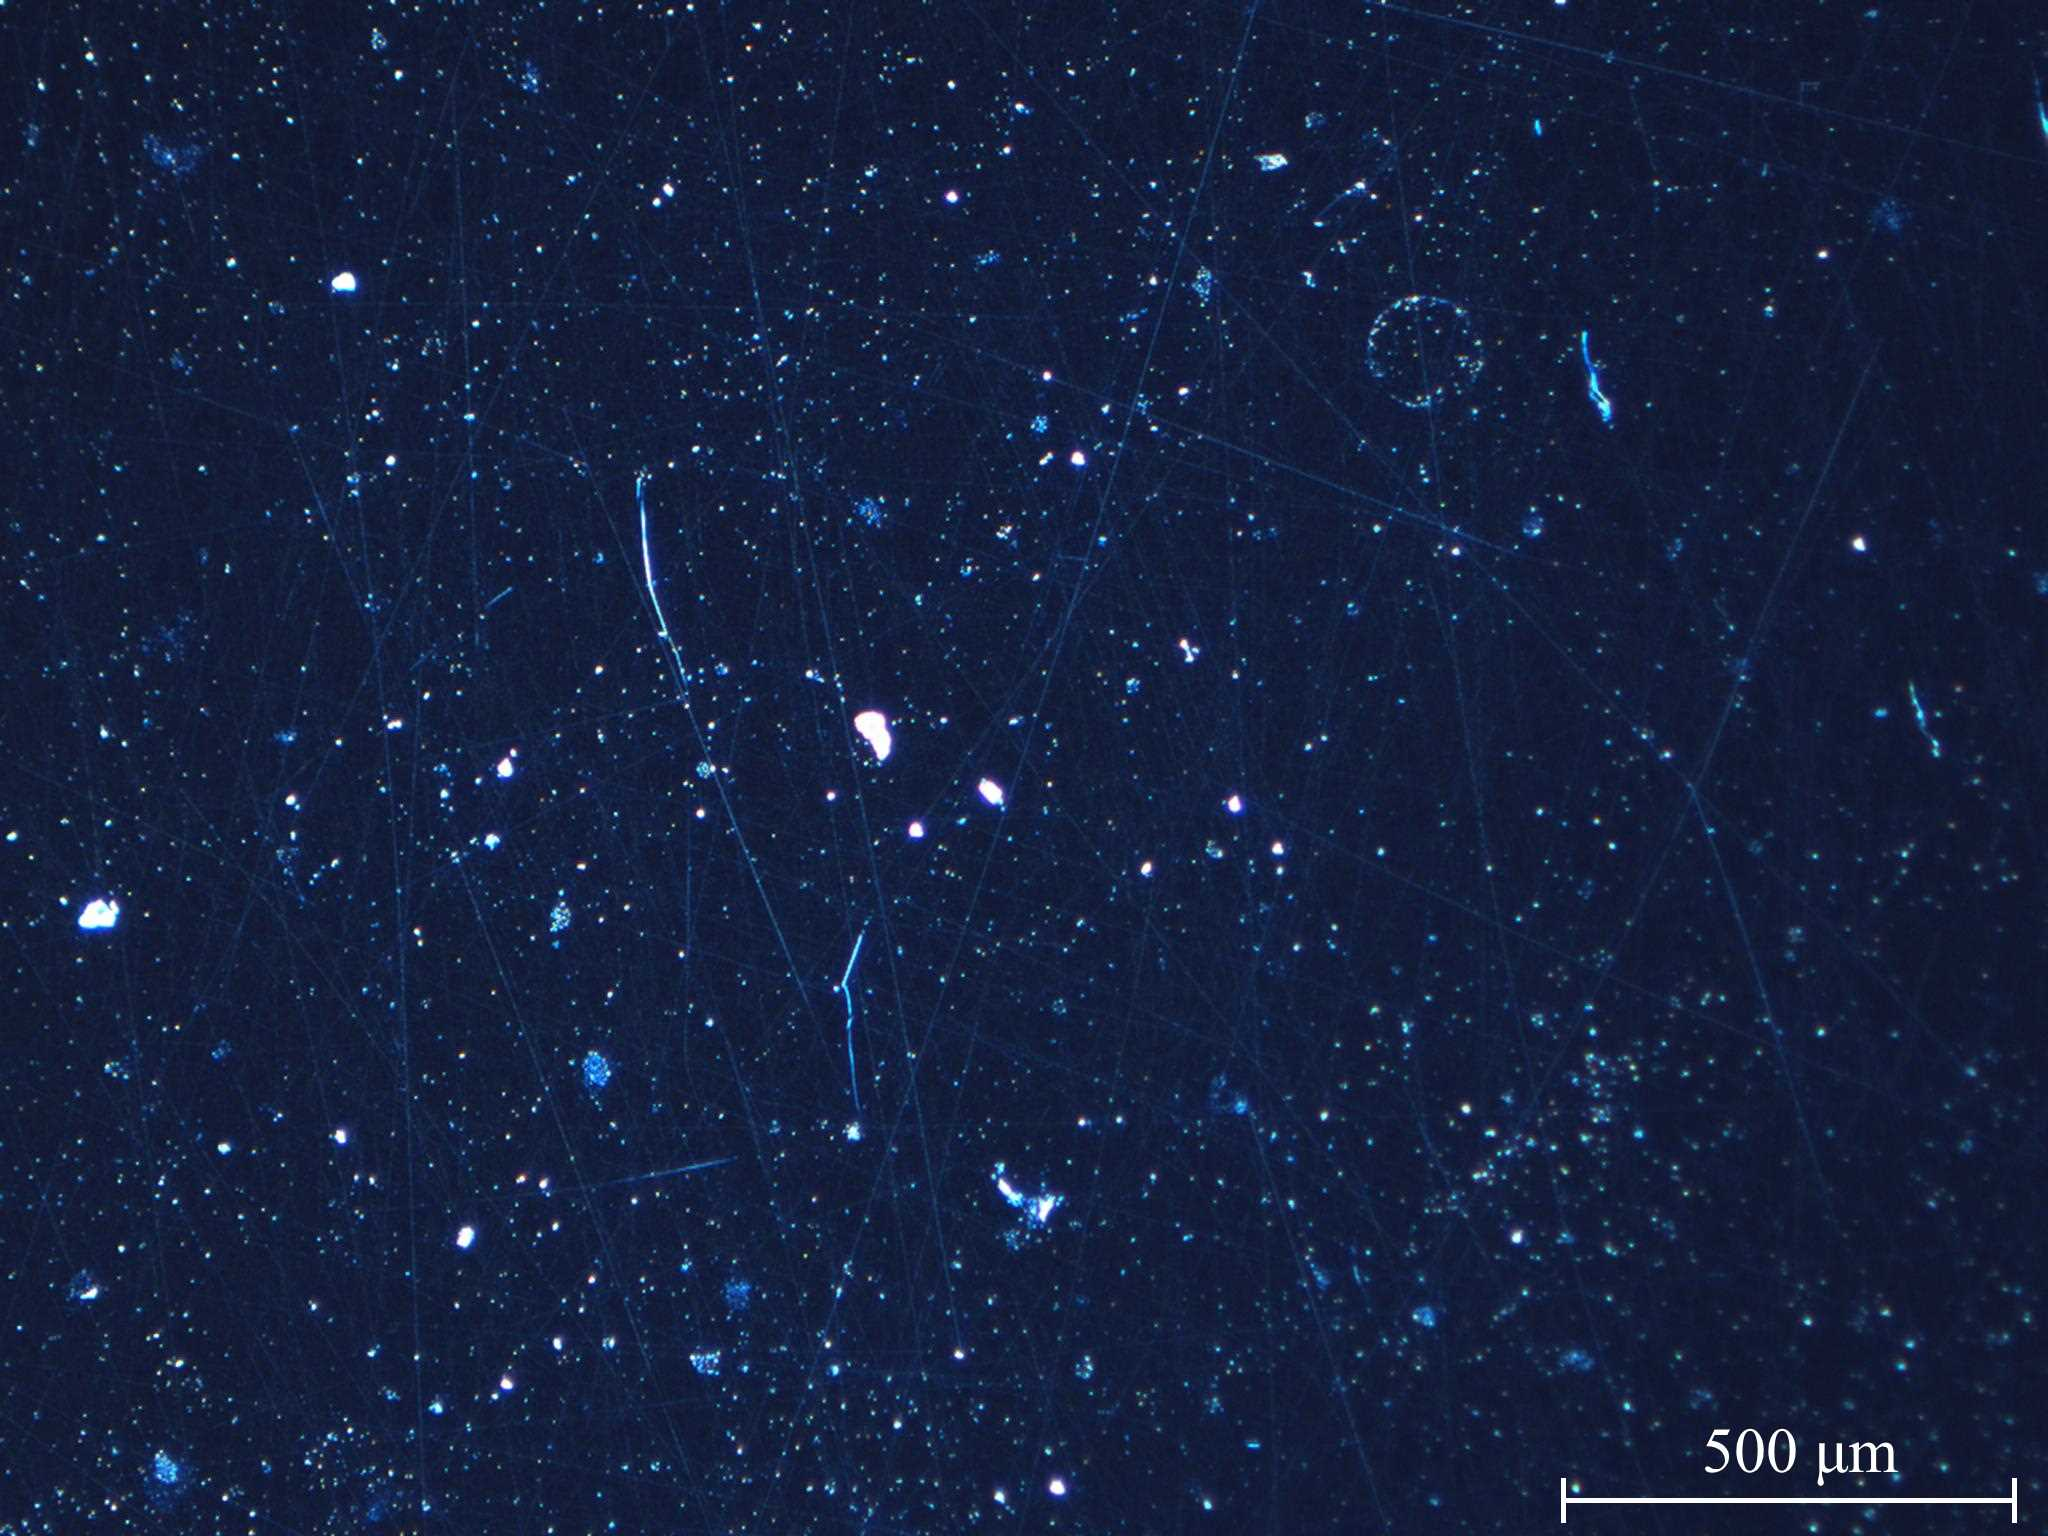
\includegraphics[width=\linewidth]{LM_DF_C389523A_M005_centre.jpg}
    %\mySubfigure{\linewidth}{LM_DF_C389523A_M005_centre.jpg}[fig:subBa_om_df_centre]
    %\par\bigskip
    %\mySubfigure{0.49\linewidth}{LM_DF_C389523A_M005_centreEdge.jpg}[fig:subBa_om_df_edge]
    %\hfill
    %\mySubfigure{0.49\linewidth}{LM_DF_C389523A_M005_corner.jpg}[fig:subBa_om_df_corner]
    \caption[Dark field images of substrate B.]{Dark field images of substrate B captured through the optical microscope Leica DM RXA2 at the centre of the substrate.}%\subref{fig:subBa_om_df_centre} centre; \subref{fig:subBa_om_df_edge} edge; and \subref{fig:subBa_om_df_corner} corner of the substrate
    \label{fig:subBa_om_df}
\end{figure}

The surface of the as-received substrate B looked completely different from that of the as-received substrate A. Fig.~\ref{fig:subBa_om_df} shows typical dark field images from the surface of substrate B at the corner, edge, and centre of the substrate. There were polishing scratches in all directions and with varying width covering the surface of substrate B. Particles and morphological defects with both small (\SIrange{0.5}{5}{\micro\metre}) and large (\SIrange{5}{50}{\micro\metre}) diameter were present on the surface. By counting the number of bright spots in the dark field image, the density of particle and morphological defects with features \SI{>0.5}{\micro\metre} was estimated to be \SI{1e5}{\centi\metre^{-2}}, both at the centre and edges of the surface of substrate B.
% --- Measured with tolerance of 10 using ImageJ. One pixel are 2250/2048 um.
%       Centre: 5739 partikler på 2048x1536 --> 151151 particles per cm^2
%       Edges: 3927 partikler på 1877x1522 --> 113888 particles per cm^2
%       Corner: 5327 partikler på 1848x1486 --> 158000 particles per cm^2

The difference between substrate A and substrate B was significant. Substrate B had a density of particles and morphological defects that was 100-1000 times larger than on substrate A. A large part of this can presumably be explained by the more thorough surface preparation that substrate A had been subjected to. Substrate A had a final polishing and an etch before it was delivered, while substrate B was roughly polished and particles on the surface had not been removed.

A comparison between the dark field image and a \ac{sem} image of the same area of substrate B, as seen in Fig.~\ref{fig:LM_SEM_C3895}, reveals that the brightest spots in the dark field image are from cavities in the substrate surface and that particles as small as \SI{0.5}{\micro\metre} can be seen in the dark field image. The dark stains, on the other hand, were not visible in the dark field image. This indicates that the dark stains do not have sharp edges or other pointy features.

\begin{figure}[htbp]
    \centering
    %\mySubfigure[Dark field optical microscope image.]{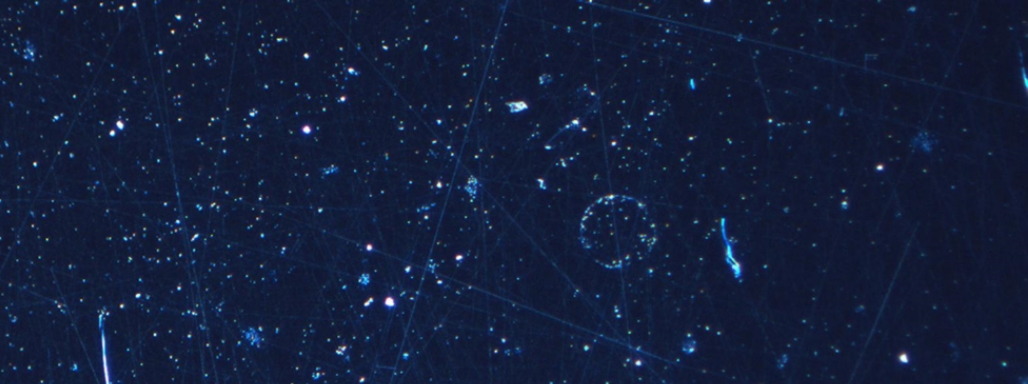
\includegraphics[width=1\linewidth]{C-3895-23A_centre_LM.jpg}\label{fig:C-3895-23A_centre_LM}}
    %\mySubfigure[SEM image at a magnification of 60$\times$.]{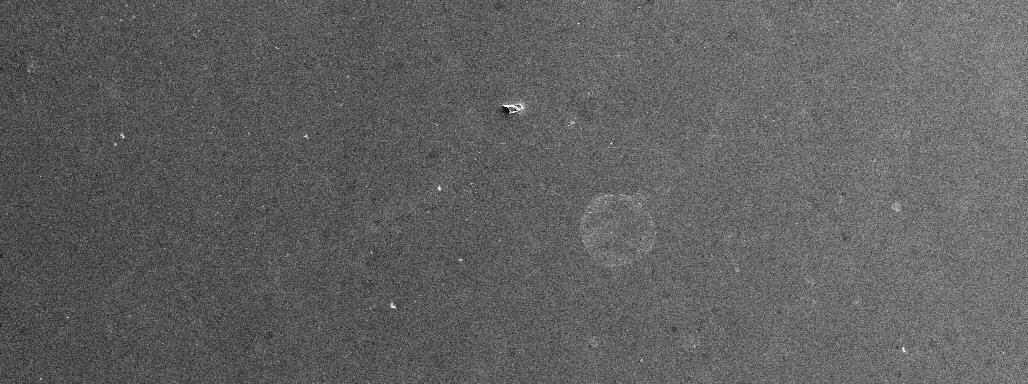
\includegraphics[width=1\linewidth]{C-3895-23A_centre_SEM.jpg}\label{fig:C-3895-23A_centre_SEM}}
    \mySubfigure{0.36\linewidth}{C-3895-23A_edge_LM_500_overview.jpg}[fig:C-3895-23A_edge_LM_500_overview]
    \hfill
    \mySubfigure{0.60\linewidth}{C-3895-23A_edge_SEM_500_overview.png}[fig:C-3895-23A_edge_SEM_500_overview]
    \caption[Comparison of dark field microscopy and \ac{sem} images.]{Comparison of \subref{fig:C-3895-23A_edge_LM_500_overview} a dark field microscopy image captured through the optical microscope Leica DM RXA2 and \subref{fig:C-3895-23A_edge_SEM_500_overview} \iacf{sem} image taken at the same location on the as-received substrate B as the dark field image.}
    \label{fig:LM_SEM_C3895}
\end{figure}

%A \ac{sem} image mapping of substrate B was performed at points in a grid of $11\times11$ grid points. The distance between neighbouring points was \SI{2.60}{\milli\metre} and the distance from the edge to the outer points was \SI{2.00}{\milli\metre}. A low magnification \ac{sem} image (60$\times$) and a higher magnification image (500$\times$) were acquired at every grid point. %This mapping will be used in future studies of substrate B when correlation between defect density and preparation methods is going to be measured.

%A particle and morphological defect density of features \SI{>0.5}{\micro\metre} of \SI{1e5}{\centi\metre^{-2}} at both the centre and at the edges of the substrate was observed. Substrate B had polishing scratches that were between 10 and \SI{100}{\nano\metre} wide. A large amount of voids with sizes ranging from \SI{5}{} to \SI{100}{\micro\metre} were observed on the surface of substrate B. 

%Most of the particles \SI{>1}{\micro\metre} on the surface of substrate B were \ce{CdZnTe} particles with lengths of between \SI{50}{} and \SI{100}{\micro\metre} that could be debris from the cutting of the substrate, but some carbon based particles was also observed with lengths of \SI{25}{\micro\metre}. Most of the particles \SI{<1}{\micro\metre} on the surface of substrate B were residual \ce{Al2O3} and \ce{SiO2} polishing grit with diameter of between \SI{50}{} and \SI{100}{\nano\metre}.  In addition, iron particles, which could be possible remainders of polishing slurry, and particles containing \ce{Na} and \ce{Cl}, which could be possible remainders of polishing slurry cleaner, were observed on the surface of substrate B.

%%=========================================
%\section{Particles and Defects on Substrate B}

Fig.~\ref{fig:C-3895-23A_F08_x060} shows a \ac{sem} image from the centre of substrate B, taken at low magnification (60$\times$). There were some bright stains at the top of the image, a dark spot down in the right corner, and several bright spots distributed over the surface. A \ac{sem} image at the same position at magnification 500$\times$, shown in Fig.~\ref{fig:C-3895-23A_F08_x500}, revealed the existence of surface scratches, dark stains of different sizes, and some even smaller bright spots on the surface. These features will be described in the following paragraphs by, among other methods, \ac{sem} images at even higher magnification.

\begin{figure}[htbp]
    \centering
    \mySubfigure{0.49\linewidth}{C-3895-23A_F08_x060.png}[fig:C-3895-23A_F08_x060]
    \hfill
    \mySubfigure{0.49\linewidth}{C-3895-23A_F08_x500.png}[fig:C-3895-23A_F08_x500]
    \caption[\Ac{sem} images of a typical area in the middle of substrate B.]{\Ac{sem} images of a typical area in the middle of substrate B at \subref{fig:C-3895-23A_F08_x060} $60\times$ magnification; and \subref{fig:C-3895-23A_F08_x500} $500\times$ magnification.}
    \label{fig:SEM_C389523_overview}
\end{figure}

\subsection{Particles and Surface Features}

Seven different types of particles and surface features were observed on the surface of substrate B. These seven can be seen in Fig.~\ref{fig:subBa_sem_w_eds}.
%\mySubfigure[SEM.]{0.44\linewidth}{C-3895-23_09_m001.jpg}
    %\mySubfigure[SEM.]{0.44\linewidth}{C-3895-23A_edx7_m002.jpg}
    %\mySubfigure[SEM.]{0.44\linewidth}{C-3895-23A_edx7_m003.jpg}
\begin{figure}[htbp]
    \centering
    \begin{subfigure}[t]{\textwidth}
        \caption{}\label{fig:subBa_polishing-grit_alumina}
          \begin{minipage}[c]{0.43\linewidth}
            \centering
            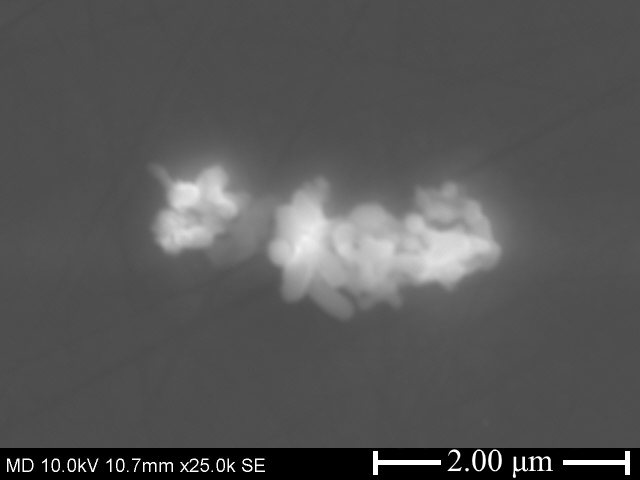
\includegraphics[width=\linewidth]{alumina02_sem.png}
          \end{minipage}
          \hfill
          \begin{minipage}[c]{0.43\linewidth}
            \centering
            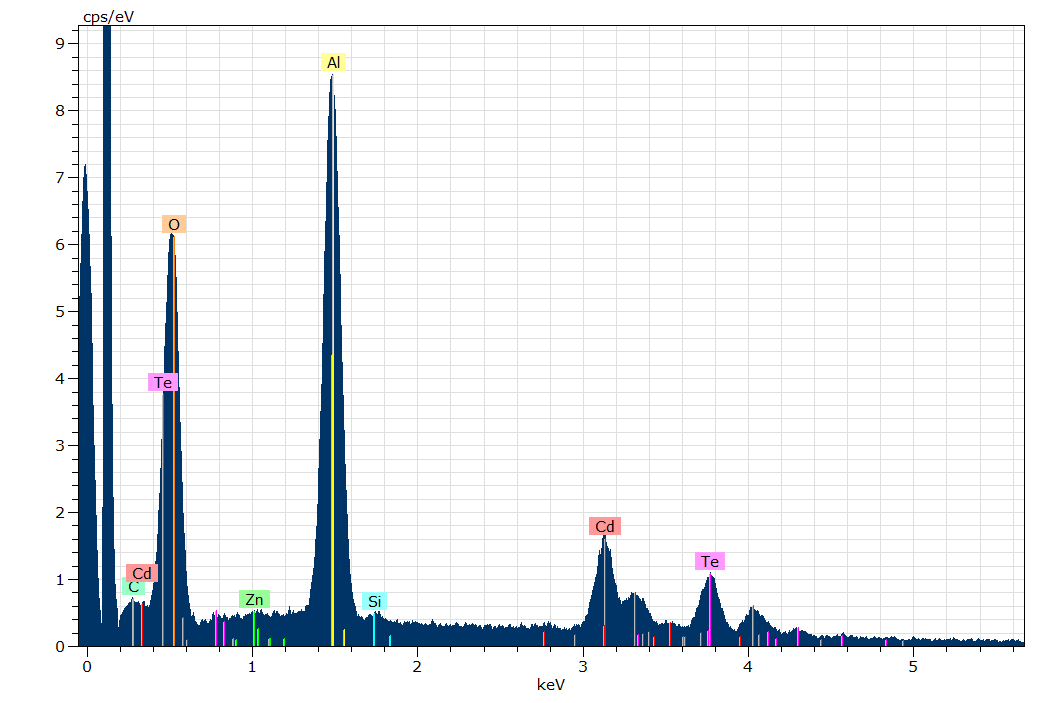
\includegraphics[width=\linewidth]{alumina02_eds.png}
          \end{minipage}
          \begin{minipage}[c]{0.11\linewidth}
            \centering
            \atomicTable[\ce{O}&\SI{46.76}{}][\ce{Al}&\SI{29.78}{}][\ce{C}&\SI{12.14}{}][\ce{Cd}&\SI{5.59}{}][\ce{Te}&\SI{5.05}{}][\ce{Si}&\SI{0.62}{}][\ce{Zn}&\SI{0.04}{}]
          \end{minipage}
    \end{subfigure}%
    \par\bigskip
    \begin{subfigure}[t]{\textwidth}
        \caption{}\label{fig:subBa_polishing-grit_silica}
          \begin{minipage}[c]{0.43\linewidth}
            \centering
            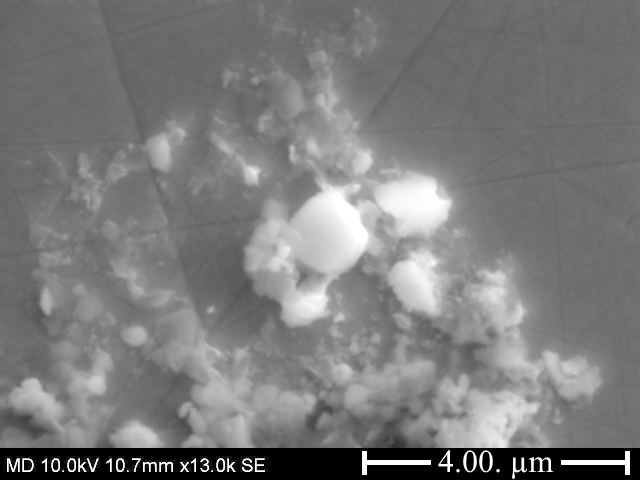
\includegraphics[width=\linewidth]{subB_silica_sem.png}
          \end{minipage}
          \hfill
          \begin{minipage}[c]{0.43\linewidth}
            \centering
            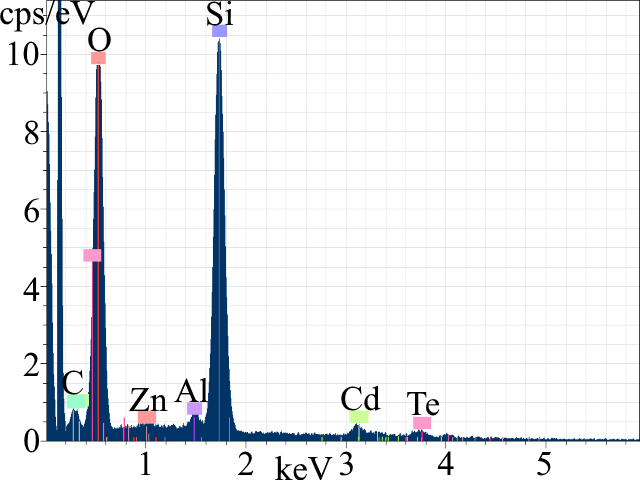
\includegraphics[width=\linewidth]{subB_silica_eds.png}
          \end{minipage}
          \begin{minipage}[c]{0.11\linewidth}
            \centering
            \atomicTable[\ce{O}&\SI{60.33}{}][\ce{Si}&\SI{22.62}{}][\ce{C}&\SI{15.45}{}][\ce{Al}&\SI{0.60}{}][\ce{Te}&\SI{0.47}{}][\ce{Cd}&\SI{0.33}{}][\ce{Zn}&\SI{0.21}{}]
          \end{minipage}
    \end{subfigure}%
    \par\bigskip
    \begin{subfigure}[t]{\textwidth}
        \caption{}\label{fig:SEM_B_particulates_eds}
          \begin{minipage}[c]{0.43\linewidth}
            \centering
            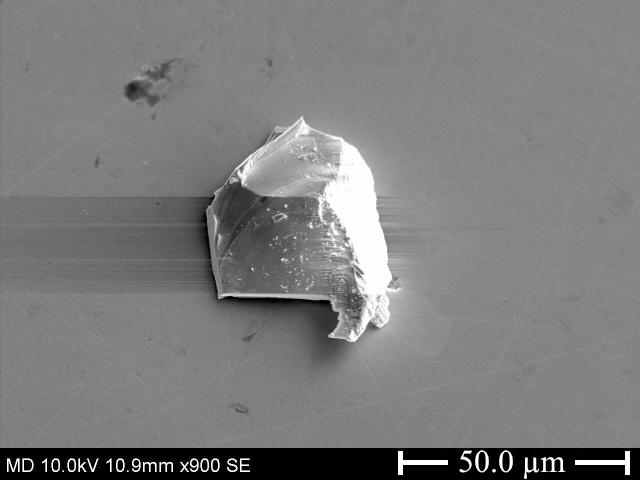
\includegraphics[width=\linewidth]{C-3895-23A_edx1_m006.png}
          \end{minipage}
          \hfill
          \begin{minipage}[c]{0.43\linewidth}
            \centering
            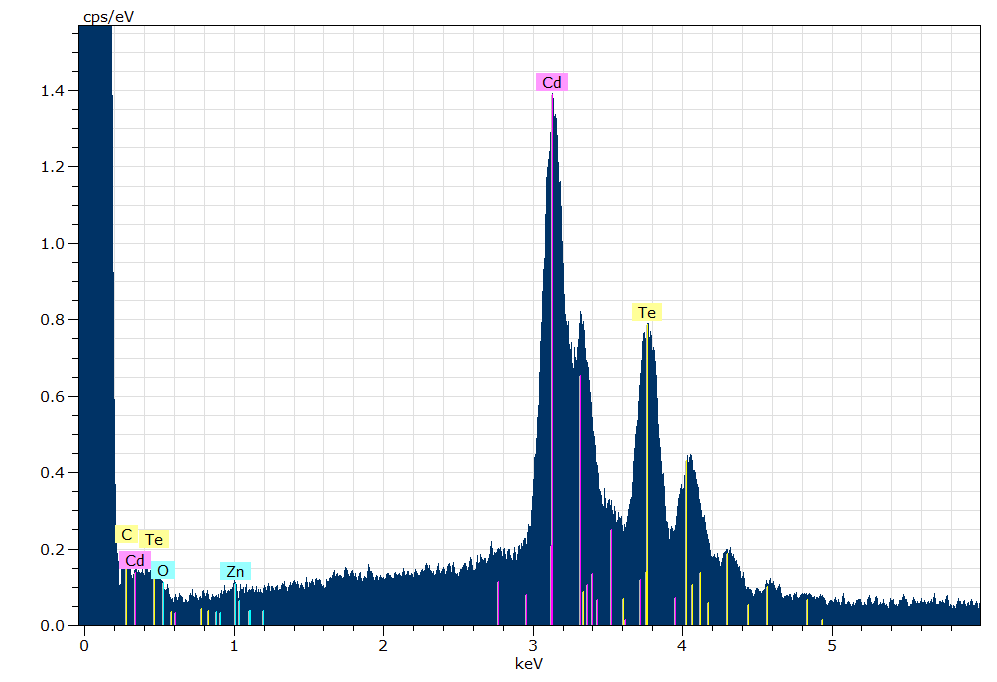
\includegraphics[width=\linewidth]{C-3895-23A_edx1_m006_eds.png}
          \end{minipage}
          \begin{minipage}[c]{0.11\linewidth}
            \centering
            \atomicTable[\ce{Cd}&\SI{46.85}{}][\ce{Te}&\SI{42.07}{}][\ce{C}&\SI{7.90}{}][\ce{Zn}&\SI{1.99}{}][\ce{O}&\SI{1.20}{}]
          \end{minipage}
          %\begin{minipage}[c]{0.49\linewidth}
          %  \centering
          %  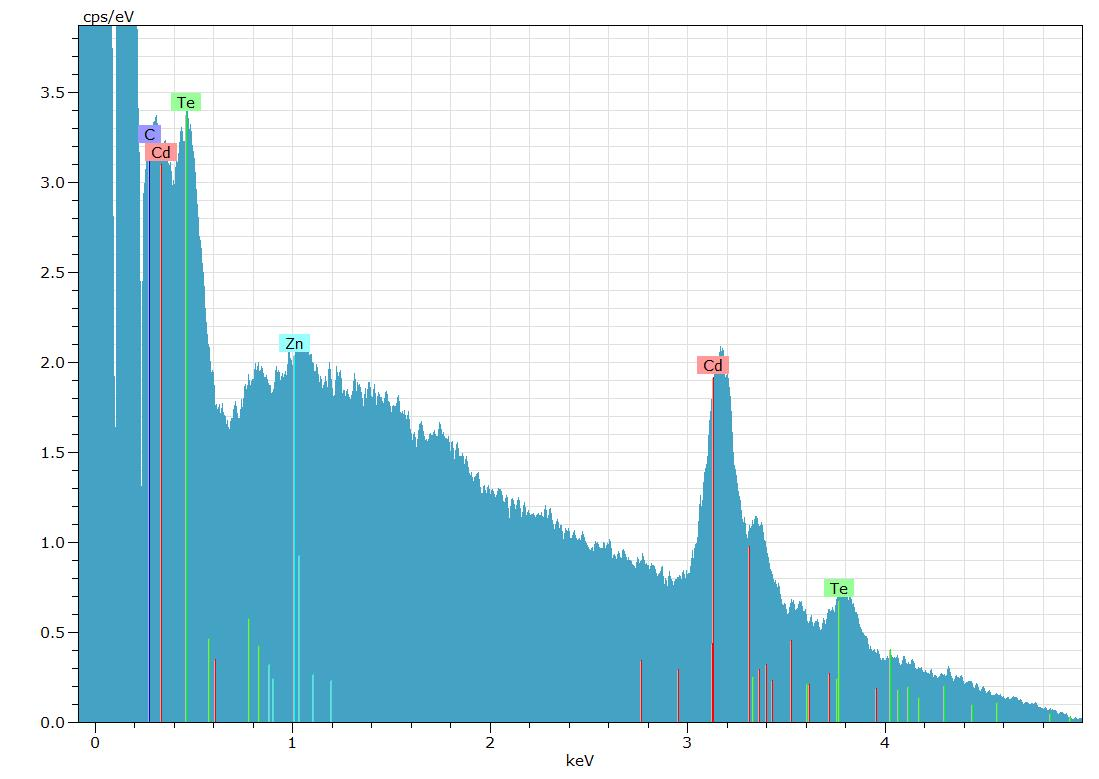
\includegraphics[width=\linewidth]{CdZnTe_eds_substrate.jpg}
          %\end{minipage}
    \end{subfigure}%
    \caption[\Ac{sem} images, \ac{eds} spectra, and \ac{eds} atomic compositions of one void and six different types of particles found on as-received substrate B.]{High resolution \ac{sem} images of one void and six different types of particles found on the as-received substrate B and the corresponding \ac{eds} spectra and atomic compositions: \subref{fig:subBa_polishing-grit_alumina} alumina (\ce{Al2O3}) polishing grit; \subref{fig:subBa_polishing-grit_silica} silica (\ce{SiO2}) polishing grit; \subref{fig:SEM_B_particulates_eds} \ac{czt} paticle; \subref{fig:subBa_particle_carbon} carbon-based particle; \subref{fig:EDS_NaClO} \ce{NaClO}; \subref{fig:subBa_partice_Fe} iron (\ce{Fe}); and \subref{fig:SEM_C389523_void_eds} void.}\label{fig:subBa_sem_w_eds}
\end{figure}
%
\begin{figure}[htbp]
\ContinuedFloat
    \centering
    \begin{subfigure}[t]{\textwidth}
        \caption{}\label{fig:subBa_particle_carbon}
          \begin{minipage}[c]{0.43\linewidth}
            \centering
            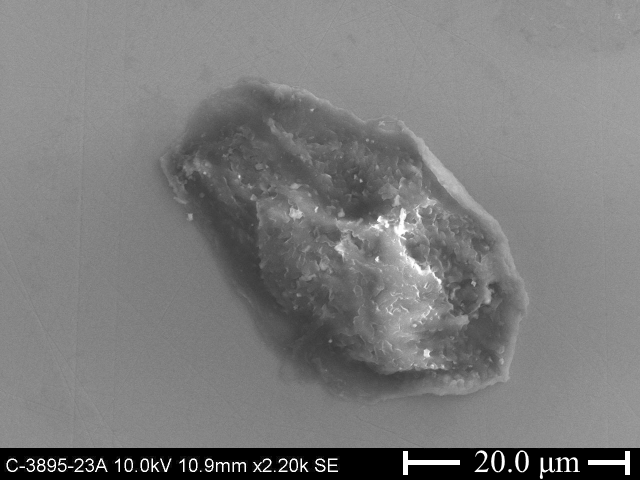
\includegraphics[width=\linewidth]{C-3895-23A_tuning_05.png}%{carbon_eds_sem.jpg} %{C-3895-23_02_m002.jpg}%{C-3895-23A_tuning_05.jpg}
          \end{minipage}
          \hfill
          \begin{minipage}[c]{0.43\linewidth}
            \centering
            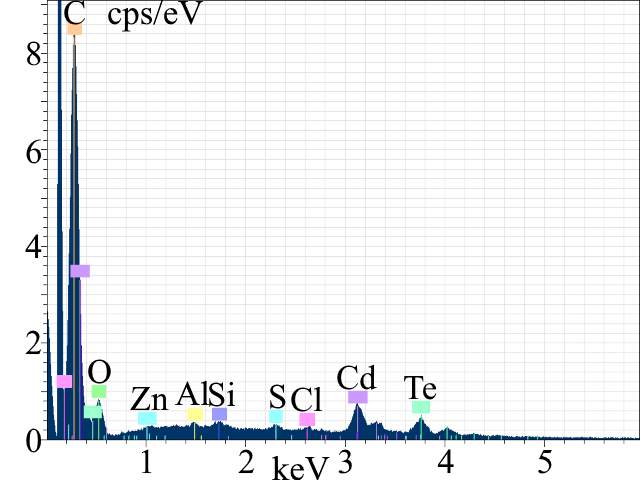
\includegraphics[width=\linewidth]{C-3895-23A_tuning_05_eds.png}
          \end{minipage}
          \begin{minipage}[c]{0.11\linewidth}
            \centering
            \atomicTable[\ce{C}&\SI{86.43}{}][\ce{O}&\SI{7.35}{}][\ce{Cd}&\SI{2.58}{}][\ce{Te}&\SI{2.06}{}][\ce{Si}&\SI{0.55}{}][\ce{S}&\SI{0.36}{}][\ce{Cl}&\SI{0.31}{}][\ce{Zn}&\SI{0.21}{}][\ce{Al}&\SI{0.15}{}]
          \end{minipage}
    \end{subfigure}%
    \par\bigskip
    \begin{subfigure}[t]{\textwidth}
    \caption{}\label{fig:EDS_NaClO}
          \begin{minipage}[c]{0.43\linewidth}
            \centering
            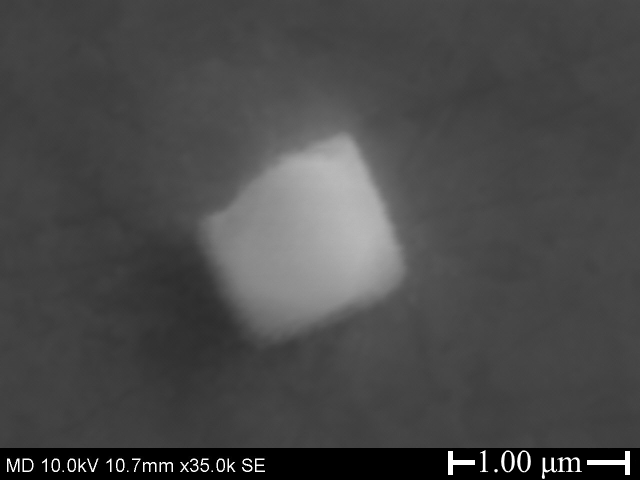
\includegraphics[width=\linewidth]{eds_NaOCl2_C-3895-23A_edx8_m007.png}
          \end{minipage}
          \hfill
          \begin{minipage}[c]{0.43\linewidth}
            \centering
            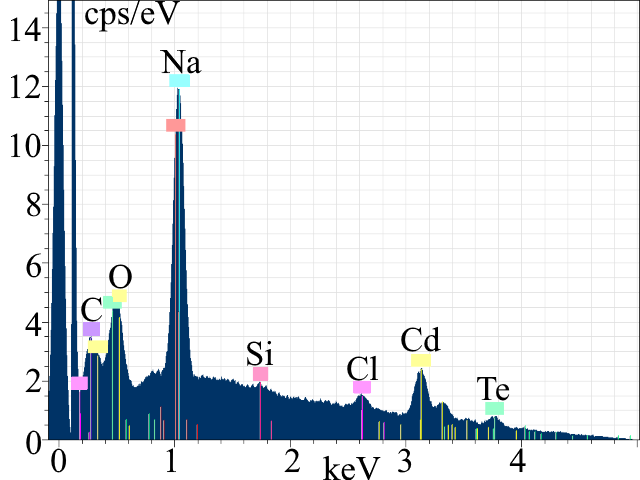
\includegraphics[width=\linewidth]{eds_NaClO2.png}
          \end{minipage}
          \begin{minipage}[c]{0.11\linewidth}
            \centering
            \atomicTable[\ce{Na}&\SI{27.17}{}][\ce{C}&\SI{22.94}{}][\ce{Te}&\SI{20.44}{}][\ce{Cd}&\SI{15.65}{}][\ce{O}&\SI{9.97}{}][\ce{Cl}&\SI{2.45}{}][\ce{Si}&\SI{0.92}{}][\ce{Zn}&\SI{0.47}{}]
          \end{minipage}
    \end{subfigure}%
    \par\bigskip
    \begin{subfigure}[t]{\textwidth}
    \caption{}\label{fig:subBa_partice_Fe}
          \begin{minipage}[c]{0.43\linewidth}
            \centering
            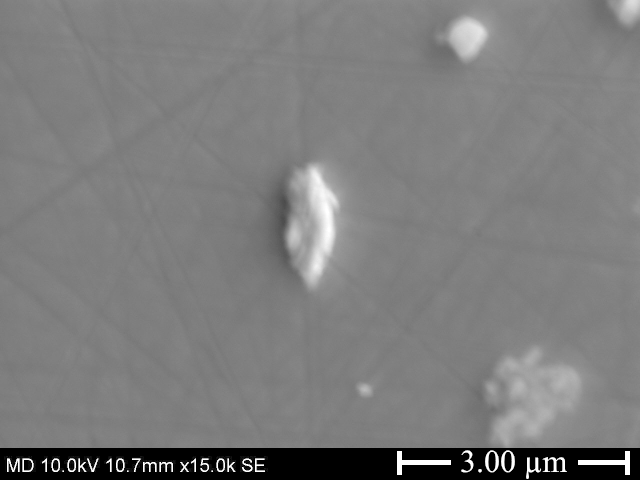
\includegraphics[width=\linewidth]{eds_Fe_C-3895-23A_edx5_m004.png}
          \end{minipage}
          \hfill
          \begin{minipage}[c]{0.43\linewidth}
            \centering
            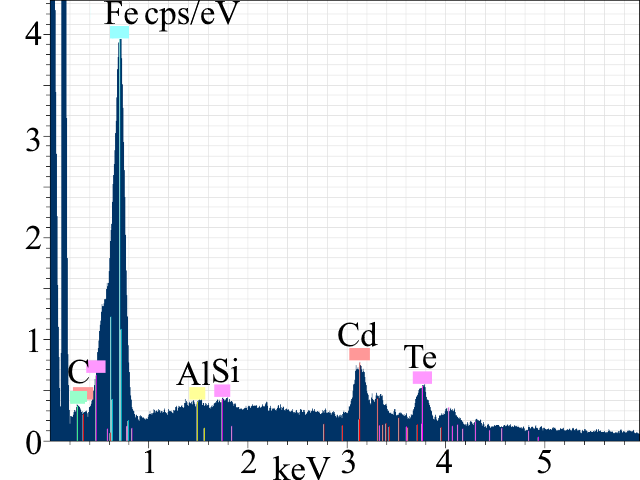
\includegraphics[width=\linewidth]{eds_Fe_C-3895-23A_edx5_m004_eds.png}
          \end{minipage}
          \begin{minipage}[c]{0.11\linewidth}
            \centering
            \atomicTable[\ce{Fe}&\SI{81.79}{}][\ce{C}&\SI{11.21}{}][\ce{Cd}&\SI{3.59}{}][\ce{Te}&\SI{3.04}{}][\ce{Si}&\SI{0.26}{}][\ce{Al}&\SI{0.11}{}]
          \end{minipage}
    \end{subfigure}%
    \captionsetup{list=no}
    \caption{\emph{(continued)}}
\end{figure}
%
\begin{figure}[htbp]
\ContinuedFloat
    \centering
    \begin{subfigure}[t]{\textwidth}
        \caption{}\label{fig:SEM_C389523_void_eds}
          \begin{minipage}[c]{0.43\linewidth}

            \centering
            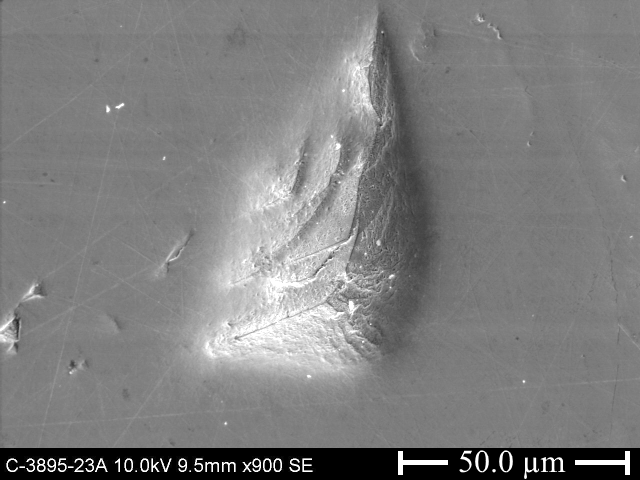
\includegraphics[width=\linewidth]{C-3895-23_09_m001.png}%C-3895-23A_edx3_m001.jpg}
          \end{minipage}
          \hfill
          \begin{minipage}[c]{0.43\linewidth}
            \centering
            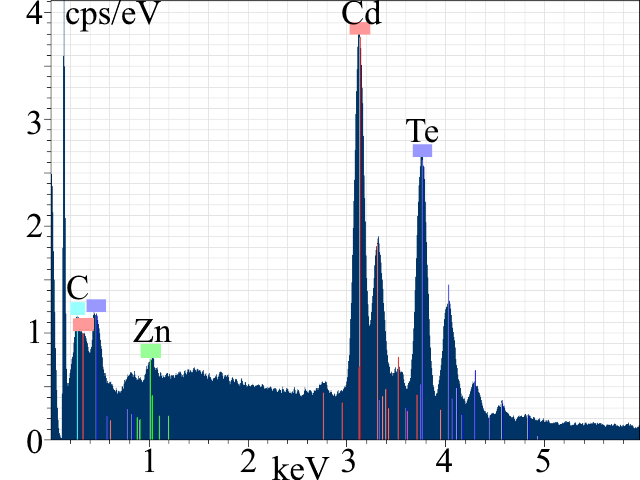
\includegraphics[width=\linewidth]{C-3895-23A_edx3_m001_eds.png}
          \end{minipage}
          \begin{minipage}[c]{0.11\linewidth}
            \centering
            \atomicTable[\ce{Te}&\SI{39.30}{}][\ce{Cd}&\SI{38.80}{}][\ce{C}&\SI{19.94}{}][\ce{Zn}&\SI{1.96}{}]
          \end{minipage}
    \end{subfigure}%
    \captionsetup{list=no}
    \caption{\emph{(continued)}}
\end{figure}

%%=====
\subsubsection{Residual Polishing Grit (alumina and silica)}
Bright particles with varying sizes were observed on the substrate surface, see Fig.~\ref{fig:subBa_polishing-grit_area1}. When looking at one of the accumulations at greater magnification, see Fig.~\ref{fig:subBa_polishing-grit_area2}, it became evident that the large particles were agglomerations of smaller particles. The smaller particles were spherical and had a diameter between \SI{50}{\nano\metre} and \SI{100}{\nano\metre}. The typical width of the particle agglomerations was \SI{0.5}{}-\SI{3}{\micro\metre}. The attraction between the small particles can be explained by electrostatic attractive forces between the particles due to different surface charge \citep{allen2001review}.

\begin{figure}[htbp]
    \centering
        \mySubfigure{0.49\linewidth}{SEM_C-3895-23A_a_m001.png}[fig:subBa_polishing-grit_area1]
        \hfill
        \mySubfigure{0.49\linewidth}{C-3895-23Ab_m003.png}[fig:subBa_polishing-grit_area2]
    \caption[\Ac{sem} images of an accumulaton of polishing grit on substrate B.]{\Ac{sem} images of an accumulation of polishing grit on the as-received substrate B at a magnification of \subref{fig:subBa_polishing-grit_area1} $200\times$ and \subref{fig:subBa_polishing-grit_area2} $15000\times$.}\label{fig:subBa_polishing-grit_area}
\end{figure}

An \ac{eds} spectrum of the particle revealed that the piece was composed of alumina oxide, \ce{Al2O3}, also known as alumina, see Fig.~\ref{fig:subBa_polishing-grit_alumina}. The corresponding \ac{sem} image of residual polishing grit is shown next to the spectrum. The presence of alumina can be explained by the frequent use of alumina as an abrasive in polishing slurries for semiconducting material. The typical density of polishing grit was \SI{6e5}{\centi\metre^{-2}}, but the density was higher near voids, deep scratches, and at stains looking like the residue after the evaporation of a droplet.

Some of the accumulations were composed of larger particles with a diameter of \SI{600}{\nano\metre} as well as the smaller ones, as seen in Fig.~\ref{fig:subBa_polishing-grit_silica}. An \ac{eds} spectrum of the largest particle revealed that the piece was composed of silicon oxide, \ce{SiO2}, also known as silica. As mentioned earlier, silica is also a frequently used abrasive in polishing slurry.

%%=====
\subsubsection{\Ac{czt}}
%Page 5-6 in eds report 1-10
Bright particles about 10 times as large as the typical polishing grit agglomerations were observed on the substrate surface, see Fig.~\ref{fig:SEM_B_particulates}. The size of the pieces was typically between \SI{50}{\micro\metre} and \SI{100}{\micro\metre}. By comparing the \ac{eds} spectrum of the particle with the spectrum of the substrate surface, see Fig.~\ref{fig:SEM_B_particulates_eds}, it became apparent that the particles had the same composition as the surrounding substrate. This indicates that the pieces could be debris from the polishing or cutting of the substrate.

\begin{figure}[htbp]
    \centering
          \begin{minipage}[c]{0.49\linewidth}
            \centering
            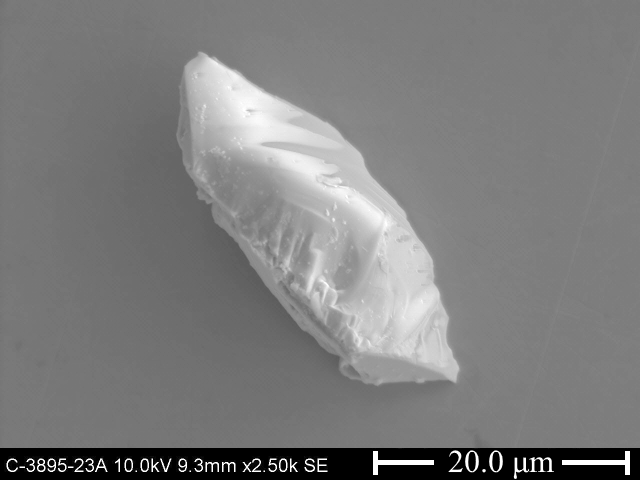
\includegraphics[width=\linewidth]{C-3895-23_03.png}
          \end{minipage}
          \hfill
          \begin{minipage}[c]{0.49\linewidth}
            \centering
            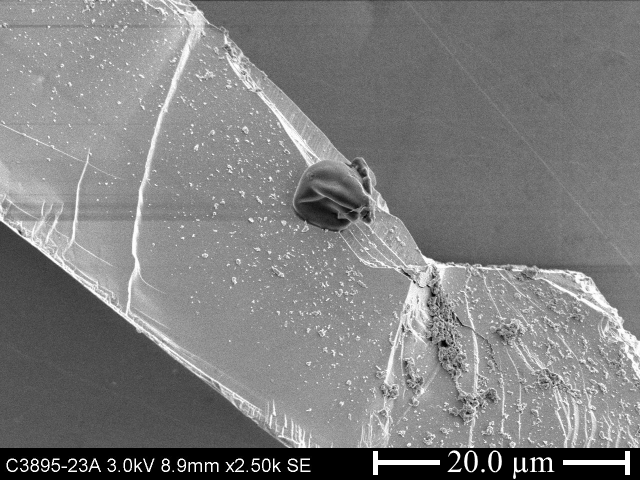
\includegraphics[width=\linewidth]{C-3895-23Af2_m002.png}
          \end{minipage}
        \caption[\Ac{sem} images of \ac{czt} particles on as-revceived substrate B.]{\Ac{sem} images of \ac{czt} particles on the as-revceived substrate B.}\label{fig:SEM_B_particulates}  
\end{figure}


%%=====
\subsubsection{Carbon-based particle}
Dark particles, which typically had a size between \SIrange{20}{30}{\micro\metre}, were observed on the substrate surface, as seen in Fig.~\ref{fig:subBa_particle_carbon}. The \ac{eds} spectrum of this particle showed a high intensity from the carbon signal. The particles could be residue from mounting wax, which was used to hold the substrate while it was being cut and polished. Some small peaks of silicon and aluminium were observed as well, but they probably stemmed from the residual polishing grit that can be seen in on the surface of the carbon-based particle.
%Page 8+12 in eds report 1-10

%%=====
\subsubsection{\ce{NaClO}}
An area with lots of circular particles with a diameter between \SI{100}{\nano\metre}--\SI{1}{\micro\metre} was observed near one of the edges of substrate B, see Fig.~\ref{fig:eds_NaOCl_overview}. The area was separated from the rest of the substrate by a dark borderline. An \ac{eds} spectrum of one particle with a diameter of \SI{1}{\micro\metre}, see Fig.~\ref{fig:EDS_NaClO}, reveals that the particle consists of \ce{Na}, \ce{Cl}, and \ce{O}. The particles could be \ce{NaClO} which typically is used after polishing as a standard cleaner to remove polishing slurry particles \citep{benson2015as-received}. The dark borderline was not possible to get quantified with \ac{eds}, but it could be a residue of the cleaning solution.

\begin{figure}[htbp]
    \centering
    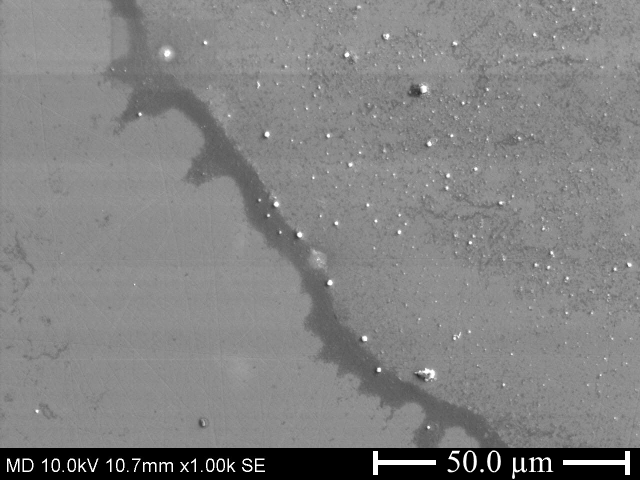
\includegraphics[width=0.48\linewidth]{eds_NaOCl_overview_C-3895-23A_edx8_m008.png}
    \caption[\Ac{sem} image of \ce{NaClO} particles on substrate B.]{\Ac{sem} image of \ce{NaClO} particles on substrate B.}
    \label{fig:eds_NaOCl_overview}
\end{figure}

%%=====
\subsection{Iron Particle}
A small particle that was \SI{1.5}{\micro\metre} long and \SI{0.6}{\micro\metre} wide can be seen in Fig.~\ref{fig:subBa_partice_Fe} with its corresponding \ac{eds} spectrum. The \ac{eds} spectrum of the particle revealed that the particle consisted mainly of \ce{Fe}. Iron is a potential contaminate in polishing grit slurry, but it could also originate in cross-contamination from the polishing of other semiconductors, i.e. \ce{InP} \citep{benson2015as-received}.

%%=====
\subsubsection{Voids}
%Page b1 in eds report 1-10
Irregular shaped voids were observed all over the surface of substrate B, see Fig.~\ref{fig:SEM_C389523_voids}. The width of the voids tended to be between \SIrange{5}{100}{\micro\metre} and \ac{afm} measurements gave that the voids were between \SIrange{1}{3}{\micro\metre} deep, see Fig.~\ref{fig:subBa_afm_voids}. \Ac{eds} detected \ce{Cd_{0.96}Zn_{0.04}Te} both on the inside edges of the voids and around the voids, see Fig.~\ref{fig:SEM_C389523_void_eds}. This revealed that the voids had the same composition as the substrate surface.

\begin{figure}[htbp]
    \centering
    \begin{subfigure}[t]{\textwidth}
    \caption{}\label{fig:subBa_voids}
          \begin{minipage}[c]{0.49\linewidth}
            \centering
            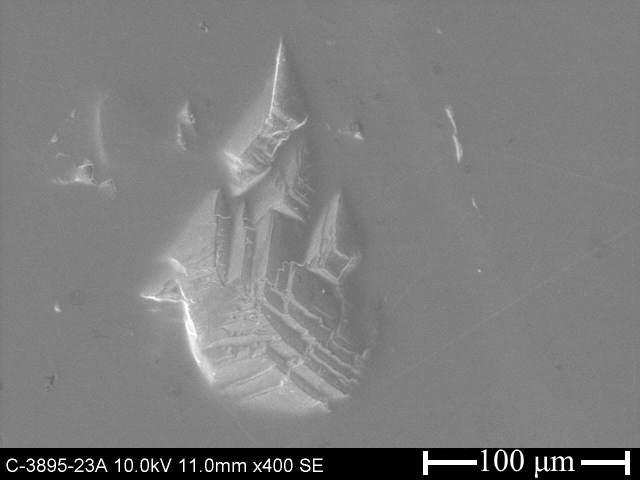
\includegraphics[width=\linewidth]{C-3895-23A_tuning_04.png}
          \end{minipage}
          \hfill
          \begin{minipage}[c]{0.49\linewidth}
            \centering
            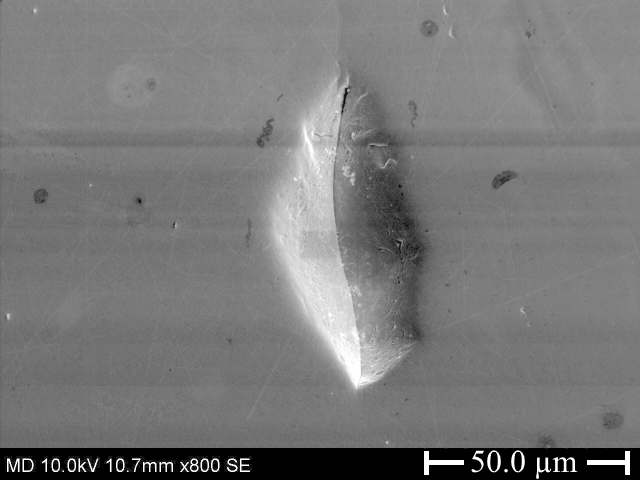
\includegraphics[width=\linewidth]{C-3895-23A_edx3_m002.png}
          \end{minipage}
    \end{subfigure}%
    \par\bigskip
    %\mySubfigure[SEM.]{0.44\linewidth}{C-3895-23A_edx7_m002.jpg}
    %\mySubfigure[SEM.]{0.44\linewidth}{C-3895-23A_edx7_m003.jpg}
    \begin{subfigure}[t]{\textwidth}
    \caption{}\label{fig:subBa_microvoids}
          \begin{minipage}[c]{0.49\linewidth}
            \centering
            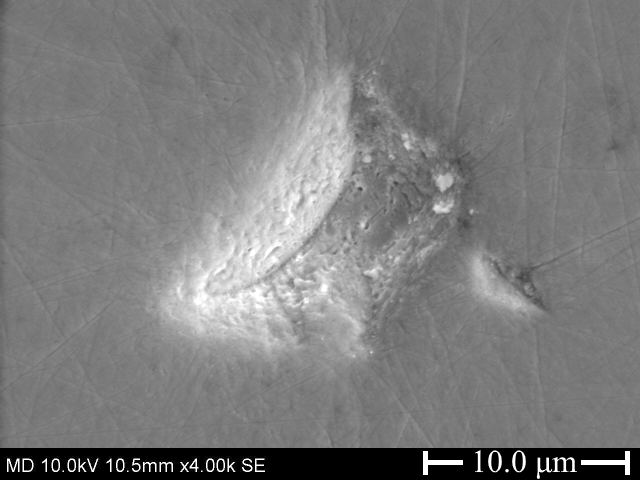
\includegraphics[width=\linewidth]{C-3895-23A_edx7_m004.png}
          \end{minipage}
          \hfill
          \begin{minipage}[c]{0.49\linewidth}
            \centering
            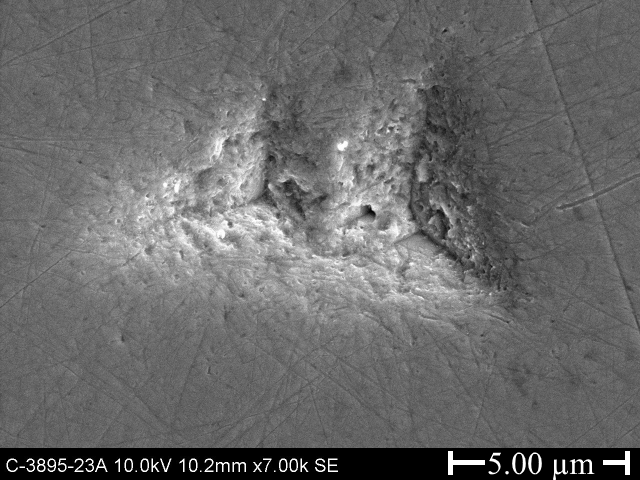
\includegraphics[width=\linewidth]{C-3895-23A_K01_detail.png}
          \end{minipage}
    \end{subfigure}%
    \caption[\Ac{sem} images of voids on substrate B.]{\Ac{sem} images of \subref{fig:subBa_voids} large voids \SI{>10}{\micro\metre} and \subref{fig:subBa_microvoids} small voids \SI{<10}{\micro\metre} on the as-received substrate B.}
    \label{fig:SEM_C389523_voids}
\end{figure}

\begin{figure}
    \centering
    \begin{subfigure}[c]{0.032\linewidth}
        \label{fig:subBa_afm_voids_scale}\captionsetup{list=no}
        
\includegraphics[width=\linewidth]{subBa_afm_voids_scale.png}
    \end{subfigure}
    \hfill
    \mySubfigure{0.46\linewidth}{subBa_afm_void_170201Topography013.png}[fig:subBa_afm_void]
    \hfill
    \mySubfigure{0.46\linewidth}{subBa_afm_microvoid_170201Topography005.png}[fig:subBa_afm_microvoid]
    \caption[\Ac{afm} measurements of voids on as-received substrate B.]{\Ac{afm} measurements of \subref{fig:subBa_afm_void} a \SI{40}{\micro\metre} wide void and \subref{fig:subBa_afm_microvoid} a \SI{7}{\micro\metre} wide void on the as-received substrate B displayed as images of $\SI{50}{\micro\metre}\times\SI{50}{\micro\metre}$ and $\SI{10}{\micro\metre}\times\SI{10}{\micro\metre}$ areas respectively.}
    \label{fig:subBa_afm_voids}
\end{figure}

\begin{figure}[htbp]
    \centering
        \mySubfigure{0.403\linewidth}{subBa_densityData.png}[fig:subBa_densityData_void_map]
        \hfill
        \mySubfigure{0.577\linewidth}{C-3895-23A_A01_x060.png}[fig:subBa_densityData_void_sem]
    \caption[Map of the void density on the as-received substrate B.]{\subref{fig:subBa_densityData_void_map} A map of the void density at 36 different locations on the as-received $\SI{30}{\milli\metre}\times\SI{30}{\milli\metre}$ substrate B. The density measurements were obtained by counting the number of voids in \ac{sem} images covering $\SI{254}{\micro\metre}\times\SI{178}{\micro\metre}$ areas. In total, \SI{0.2}{\percent} of the substrate surface was measured. The void density was observed to vary between \SIrange{2e+03}{2e+4}{\centi\metre^{-2}}. \subref{fig:subBa_densityData_void_sem} An image from the upper right corner of the grid where the void density is highest.}
    \label{fig:subBa_densityData_voids}
\end{figure}

Some of the smaller voids have a threefold symmetry, as seen in Fig.~\ref{fig:subBa_microvoids}. The larger voids \SI{>10}{\micro\metre} tended to have multiple angular features, as seen in Fig.~\ref{fig:subBa_voids}. \citet{reddy2013cross} speculate that these voids originally was occupied by a tellurium precipitate that was knocked loose during surface preparation, i.e. substrate polishing in this case, leaving a void on the surface. This theory is supported by the fact that tellurium precipitates often are crystalline and could be the source of the angular features of the voids \citep{wang2008observation}.

The void density was found to be between \SIrange{2e+03}{2e+4}{\centi\metre^{-2}}. The average void density was \SI{7e+03}{\centi\metre^{-2}} with a standard deviation of \SI{5e+03}{\centi\metre^{-2}}. A graphical representation of the void density at different locations on substrate B can be seen in Fig.~\ref{fig:subBa_densityData_voids}.

\begin{comment}
The void density was found to be between \SI{1e+02}{\centi\metre^{-2}} and \SI{2e+3}{\centi\metre^{-2}}. The mean void density was \SI{4e+02}{\centi\metre^{-2}} with a standard deviation of \SI{3e+02}{\centi\metre^{-2}}. A graphical representation of the void density at different locations on substrate B can be seen in Fig.~\ref{fig:subBa_densityData_largevoid}.

\begin{figure}[htbp]
    \centering
        \mySubfigure{0.403\linewidth}{subBa_densityData_largevoids.png}[fig:subBa_densityData_largevoid_map]
        \hfill
        \mySubfigure{0.577\linewidth}{C-3895-23A_A01_x060.png}[fig:subBa_densityData_largevoid_sem]
    \caption[Map of the large void density on the as-received substrate B.]{\subref{fig:subBa_densityData_void_map} A map of the large void density at 36 different locations on the as-received $\SI{30}{\milli\metre}\times\SI{30}{\milli\metre}$ substrate B. The large void density was observed to vary between \SI{1e+02}{\centi\metre^{-2}} and \SI{2e+3}{\centi\metre^{-2}}. \subref{fig:subBa_densityData_void_sem} An image from the upper right corner of the grid where the large void density is highest.}
    \label{fig:subBa_densityData_void}
\end{figure}

The microvoid density was found to be between \SI{2e+03}{\centi\metre^{-2}} and \SI{2e+4}{\centi\metre^{-2}}. The mean microvoid density was \SI{6e+03}{\centi\metre^{-2}} with a standard deviation of \SI{5e+03}{\centi\metre^{-2}}. A graphical representation of the microvoid density at different locations on substrate B can be seen in Fig.~\ref{fig:subBa_densityData_microvoid}.
%Voids: Minimum = 1.28e+02. Maximum = 1.91e+03. Mean = 4.20e+02. Standard deviation = 3.26e+02.
%Microvoids: Minimum = 2.21e+03. Maximum = 2.21e+04. Mean = 6.09e+03. Standard deviation = 5.06e+03

\begin{figure}[htbp]
    \centering
        \mySubfigure{0.403\linewidth}{subBa_densityData_microvoids.png}[fig:subBa_densityData_microvoid_map]
        \hfill
        \mySubfigure{0.577\linewidth}{C-3895-23A_A11_x500.png}[fig:subBa_densityData_microvoid_sem]
    \caption[Map of the microvoid density on the as-received substrate B.]{\subref{fig:subBa_densityData_microvoid_map} A map of the microvoid density at 36 different locations on the as-received $\SI{30}{\milli\metre}\times\SI{30}{\milli\metre}$ substrate B. The microvoid density was observed to vary between \SI{2e+03}{\centi\metre^{-2}} and \SI{2e+4}{\centi\metre^{-2}}. \subref{fig:subBa_densityData_microvoid_sem} An image from the upper right corner of the grid where the microvoid density is highest.}
    \label{fig:subBa_densityData_microvoid}
\end{figure}
\end{comment}

%%=====
\subsection{Circular stains}
Four typical stains that were observed on the substrate surface with \ac{sem} is shown in Fig.~\ref{fig:subB_stains}. One type of stain had a bright background with a darker centre in one part of the stain, as seen in Fig.~\ref{fig:EDX_C-3895-23Ad_m001}--\oldsubref{fig:EDX_C-3895-23A_edx1_m005}. The size of the bright stains varies from \SI{30}{\micro\metre} to \SI{150}{\micro\metre}. The density of this type of stain was estimated from the \ac{sem} grid map to be \SI{2e2}{\centi\metre^{-2}}. These stains could be residue from the evaporation of a droplet on the surface, with the centre consisting of the impurities that were carried by the surface tension of the droplet. %The bright background could be a thin layer of ...

\begin{figure}[htbp]
    \centering
    \mySubfigure{0.48\linewidth}{C-3895-23A_edx1_m001.png}[fig:EDX_C-3895-23Ad_m001]
    \mySubfigure{0.48\linewidth}{C-3895-23A_edx1_m005.png}[fig:EDX_C-3895-23A_edx1_m005]
    \par\bigskip
    \mySubfigure{0.48\linewidth}{C-3895-23A_edx1_m003.png}[fig:EDX_C-3895-23A_edx1_m003]
    \mySubfigure{0.48\linewidth}{C-3895-23A_edx1_m016.png}[fig:EDX_C-3895-23A_edx1_m016]
    \caption[\Ac{sem} images of stains on substrate B.]{\Ac{sem} images of \subref{fig:EDX_C-3895-23Ad_m001}--\subref{fig:EDX_C-3895-23A_edx1_m005} bright and \subref{fig:EDX_C-3895-23A_edx1_m003}--\subref{fig:EDX_C-3895-23A_edx1_m016} dark stains on substrate B.}
    \label{fig:subB_stains}
\end{figure}

A second type of stain, as seen Fig.~\ref{fig:EDX_C-3895-23A_edx1_m003}, appeared dark in the \ac{sem} images and had sizes ranging between \SIrange{8}{15}{\micro\metre}. The density of these stains was estimated from the \ac{sem} grid map to be \SI{1e3}{\centi\metre^{-2}}. The third type of stain appeared as a dark shadow on the substrate surface when observed in \ac{sem}, see Fig.~\ref{fig:EDX_C-3895-23A_edx1_m016}. The typical size of these stains were \SIrange{10}{50}{\micro\metre} and the density of these stains was estimated to be \SI{1e4}{\centi\metre^{-2}}. The observed stains do not contribute any additional signal to the \ac{eds} spectrum due to their thin layer on the surface. Hence, it has not been possible to identify what the composition of the stains were. 
%Page 11 in eds report 1-10

%%=========================================
%\section{AFM Study of As-Received Substrate B}
\subsection{Surface Scratches and Roughness}
The surface of substrate B had been subjected to a coarse polish, and scratches stemming from the polishing could be seen on the surface. The scratches were typically between \SIrange{10}{100}{\nano\metre} wide, as seen in Fig.~\ref{fig:C-3895-23Ad_m002}. Some large scratches were located close to the edges and were as wide as \SI{1}{\micro\metre}, as seen in Fig.~\ref{fig:C-3895-23A_J08_detail}. The latter were not as evenly distributed as the polishing scratches. These types of scratches are typical of handling tools, i.e. the teflon tweezers, and could be caused by the vendor or by the handling at \ac{ffi}. The surface scratches on substrate B are most likely deeper than those on substrate A since they are visible on the dark field images of substrate B, see Fig.~\ref{fig:subBa_om_df}. Substrate B needs a fine polishing before growth to get rid of the scratches.
\begin{figure}[htbp]
    \centering
    \mySubfigure{0.48\linewidth}{C-3895-23Ad_m002.png}[fig:C-3895-23Ad_m002]
    \mySubfigure{0.48\linewidth}{C-3895-23A_J08_detail.png}[fig:C-3895-23A_J08_detail]
    \caption[\Ac{sem} images of scratches on substrate B.]{\Ac{sem} images of \subref{fig:C-3895-23Ad_m002} polishing scratches and \subref{fig:C-3895-23A_J08_detail} deep scratches on substrate B.}
    \label{fig:SEM_C389523_scratches}
\end{figure}

\begin{figure}[htbp]
    \centering
    \begin{subfigure}[c]{0.032\linewidth}
        \label{fig:subBa_afm_scale}\captionsetup{list=no}
        
\includegraphics[width=\linewidth]{subBa_afm_scale.png}
    \end{subfigure}
    \hfill
    \mySubfigure{0.3\linewidth}{subBa_afm_centre.png}[fig:subBa_afm_centre]
    \hfill
    \mySubfigure{0.3\linewidth}{subBa_afm_leftedge.png}[fig:subBa_afm_edge]
    \hfill
    \mySubfigure{0.3\linewidth}{subBa_afm_upperleftcorner.png}[fig:subBa_afm_corner]
    \caption[\Ac{afm} of as-received substrate B.]{\Ac{afm} measurements of the as-received substrate B. Images of $\SI{5}{\micro\metre}\times\SI{5}{\micro\metre}$ areas are taken at three different locations on the substrate surface: \subref{fig:subBa_afm_centre} near the centre, \ac{rms} roughness \SI{3,7}{\nano\metre}; \subref{fig:subBa_afm_edge} near the left edge, \ac{rms} roughness \SI{4,8}{\nano\metre}; and \subref{fig:subBa_afm_corner} near the upper left corner, \ac{rms} roughness \SI{4,8}{\nano\metre}. The bright line near the top of the image is due to the tip losing track of the surface.}\label{fig:subBa_afm}
\end{figure} % AFM, substrate B, as-received.

Complementary \ac{afm} images are shown in Fig.~\ref{fig:subBa_afm} where $\SI{5}{\micro\metre}\times\SI{5}{\micro\metre}$ areas were measured at three different locations on the substrate surface: near the centre, upper edge, and upper left corner. The \ac{rms} roughness of substrate B was \SI{\sim 3.7}{\nano\metre} at the centre and \SI{\sim 4.8}{\nano\metre} around the edges and corners, which was larger than the \ac{rms} roughness measured on substrate A by a factor of \SIrange{12}{16}{}. The large \ac{rms} roughness indicates that the substrate had large scratches and was inferior to substrate A. With too large \ac{rms} roughness, the surface appears 3-dimensional instead of 2-dimensional, resulting in poorer film growth (R. Haakenaasen, personal communication, May 29, 2017). The \ac{czt} substrate surfaces are easily damaged by surface scratches caused by mechanical lapping \citep{egan2009scanning}. The final polishing step performed by the vendor had left scratches on the surface, as can be observed in all the \ac{afm} images. The largest polishing scratches on substrate B were \SI{0.3}{\micro\metre} wide and \SI{15}{\nano\metre} deep.



%%=========================================
%\section{Near-IR of As-Received Substrate B}

%%=========================================
\subsection{Impurity Analysis -- EDS}

\Ac{eds} impurity analysis was performed on the as-received substrate B. Three locations on the surface -- the centre, the edge, and the corner -- were analysed. The results of this analysis can be seen in Table~\ref{tab:subBa_eds_analysis}. The only elements found above the \ac{eds} detection limit, in addition to \ce{Cd}, \ce{Zn}, and \ce{Te}, were \ce{Al}, \ce{Si}, \ce{C}, and \ce{O}. The relative concentrations of \ce{Cd}, \ce{Zn}, and \ce{Te} had an error of less than one percentage point from the expected value of \SI{48}{\atomic\percent} cadmium, \SI{2}{\atomic\percent} zinc, and \SI{50}{\atomic\percent} tellurium. The atomic concentration of aluminium and silicon near the centre of the substrate is slightly lower compared to the concentrations near the edge and corner. The atomic concentration of silicon was twice as large as the atomic concentration of aluminium, which indicates that there was a higher occurrence of silica than alumina.

\begin{table}[htbp]
    \centering
    \caption[\Ac{eds} impurity analysis of the as-received substrate B.]{Results of the \ac{eds} impurity analysis at three different locations on the $\SI{30}{\milli\metre}\times\SI{30}{\milli\metre}$ as-received (111)B \ac{czt} substrate B (atomic concentration \%). The X-ray signal was acquired from $\SI{1270}{\micro\metre}\times\SI{890}{\micro\metre}$ areas near the centre, upper edge, and upper left corner.}\label{tab:subBa_eds_analysis}
    \begin{tabu} to 1.0\textwidth { X[1.85,r] X[1.125,c] X[1.125,c] X[1.125,c] X[1.125,c] X[1.125,c] X[1.125,c] X[1.125,c] }
    \hline
         & \textbf{\ce{Te}} (at.\%) & \textbf{\ce{Cd}} (at.\%) & \textbf{\ce{Zn}} (at.\%) & \textbf{\ce{Al} } (at.\%) & \textbf{\ce{Si}} (at.\%) & \textbf{\ce{C}} (at.\%) & \textbf{\ce{O}} (at.\%) \\ % \textbf{$X$} (\SI{}{\milli\metre}) &  \textbf{$Y$} (\SI{}{\milli\metre})
        \hline
        Near centre & \SI{45.88}{} & \SI{45.35}{} & \SI{2.13}{} & \SI{0.18}{} & \SI{0.47}{} & \SI{4.59}{} & \SI{1.40}{}  \\ %\SI{15.1}{} & \SI{15.1}{}
        Near edge & \SI{45.84}{} & \SI{45.39}{} & \SI{2.28}{} & \SI{0.21}{} & \SI{0.51}{} & \SI{4.59}{} & \SI{1.18}{}   \\ % \SI{15.1}{} & \SI{29.0}{}
        Near corner & \SI{45.86}{} & \SI{45.45}{} & \SI{2.28}{} & \SI{0.36}{} & \SI{0.49}{} & \SI{4.23}{} & \SI{1.33}{}  \\ %\SI{1.0}{}  & \SI{29.0}{}
         \hline
    \end{tabu}
\end{table}
%%========================================
% FTIR transmission spectra.
\subsection{IR Characterisation}

\Ac{ftir} transmission spectra were recorded from an $11\times11$ grid on the as-received substrate B2. The grid points were placed \SI{2.0}{\milli\metre} from the edge and had \SI{2.6}{\milli\metre} between nearest neighbours. The spectra measured in the upper half of substrate B2 had the same characteristics as substrate A, and hence, had the same properties regarding precipitates and carrier concentration as substrate A \citep{yujie2004infrared}. Some of the spectra measured in the lower half of the substrate deviated by having a downward slope for lower wavenumbers, see Fig.~\ref{fig:subB2a_ftir_spectra}. These spectra had a value of $T_{5000}$ \SI{<60}{\percent} and $T_{1000}$ \SI{\ll 60}{\percent}. According to \citet{yujie2004infrared}, \ac{czt} substrates with these parameters have a higher free carrier concentration, on the order of  \SI{e17}{\centi\metre^{-2}}, and a lower resistivity than the other spectra. The area of low-transmission form a semicircle in the lower part of substrate B2, as seen in Fig.~\ref{fig:subB2a_ftir_map_500cm-1}. %\todo{Why resisitivity?} % and resistivity of the order \SI{e2}{\ohm\centi\metre} Aa: e6 ohm centi metre

\begin{figure}[htbp]
    \centering
    \mySubfigure{0.60175438596\linewidth}{subB2a_121_ftir_spectra.png}[fig:subB2a_ftir_spectra]
    \hfill
    \mySubfigure{0.37824561403\linewidth}{subB2a_121_ftir_transmission_at_k500cm-1.png}[fig:subB2a_ftir_map_500cm-1]
    \caption[\Ac{ftir} measurements of the as-received substrate B2.]{\Ac{ftir} measurements recorded from a $11\times11$ grid on the as-received $\SI{30}{\milli\metre}\times\SI{30}{\milli\metre}$ (111)B-oriented substrate B2: \subref{fig:subB2a_ftir_spectra} Transmission spectra; \subref{fig:subB2a_ftir_map_500cm-1} transmission map at wavenumber $k=\SI{500}{\centi\metre^{-1}}$ showing the transmittance $T$ in percentage of incoming light at each grid point. The spikes near $k=\SI{4500}{\centi\metre^{-1}}$ and $k=\SI{5000}{\centi\metre^{-1}}$ were artefacts of the \ac{ftir} instrument.}
\end{figure}

Surprisingly, the low-transmission semicircle was visible as a brighter area in the \ac{sem} images, see Fig.~\ref{fig:subB2b_sem_low_transmission}. The semicircle started \SI{4.11}{\milli\metre} from the left edge, went around up to \SI{13.11}{\milli\metre} before it went down, and ended \SI{1.89}{\milli\metre} from the right edge. The major influence on \ac{se} generation is the topography of the surface, and generally, edges and other pointy parts that are facing the detector produce more \acp{se}, and hence, these parts look brighter than the rest of the image \citep{goldstein2012scanning}. This was not the case for the brighter area because \ac{afm} measurements affirmed that the surface was as uniform and planar as the surrounding substrate. Also, the average atomic number influences the contrast, but \ac{eds} spectra confirmed that the low-transmission area and the surrounding substrate had the same composition.

\begin{figure}[htbp]
    \centering
    \mySubfigure{0.49\linewidth}{subB2b_sem_04_m007.png}[fig:subB2b_sem_low_transmission_left]
    \hfill
    \mySubfigure{0.49\linewidth}{subB2b_sem_04_m005.png}[fig:subB2b_sem_low_transmission_right]
    %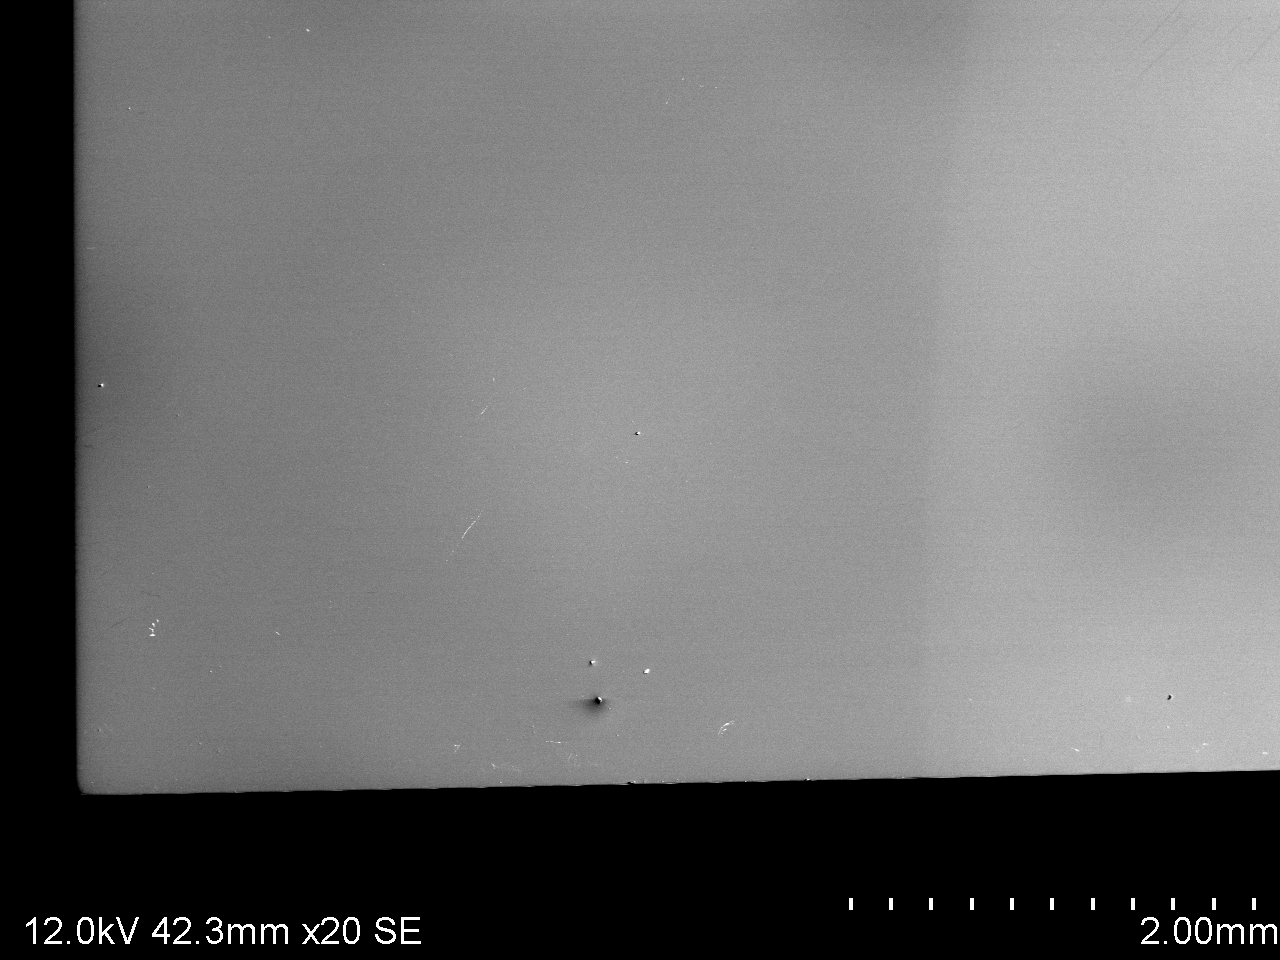
\includegraphics[width=1.0\linewidth]{subB2b_sem_05_m002.png}\caption{Left edge}
    %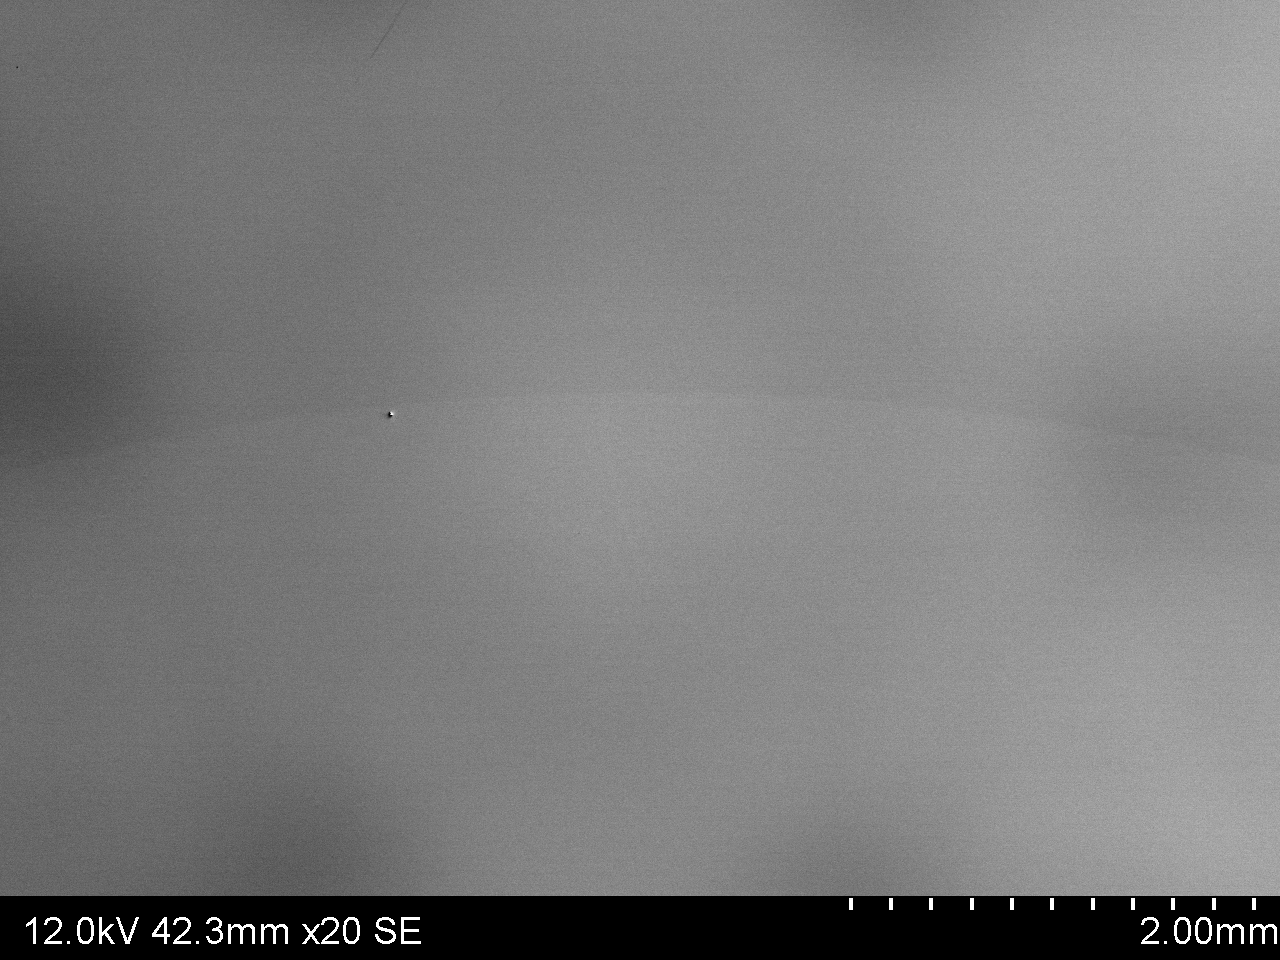
\includegraphics[width=1.0\linewidth]{subB2b_sem_05_m005.png}\caption{Upper edge}
    %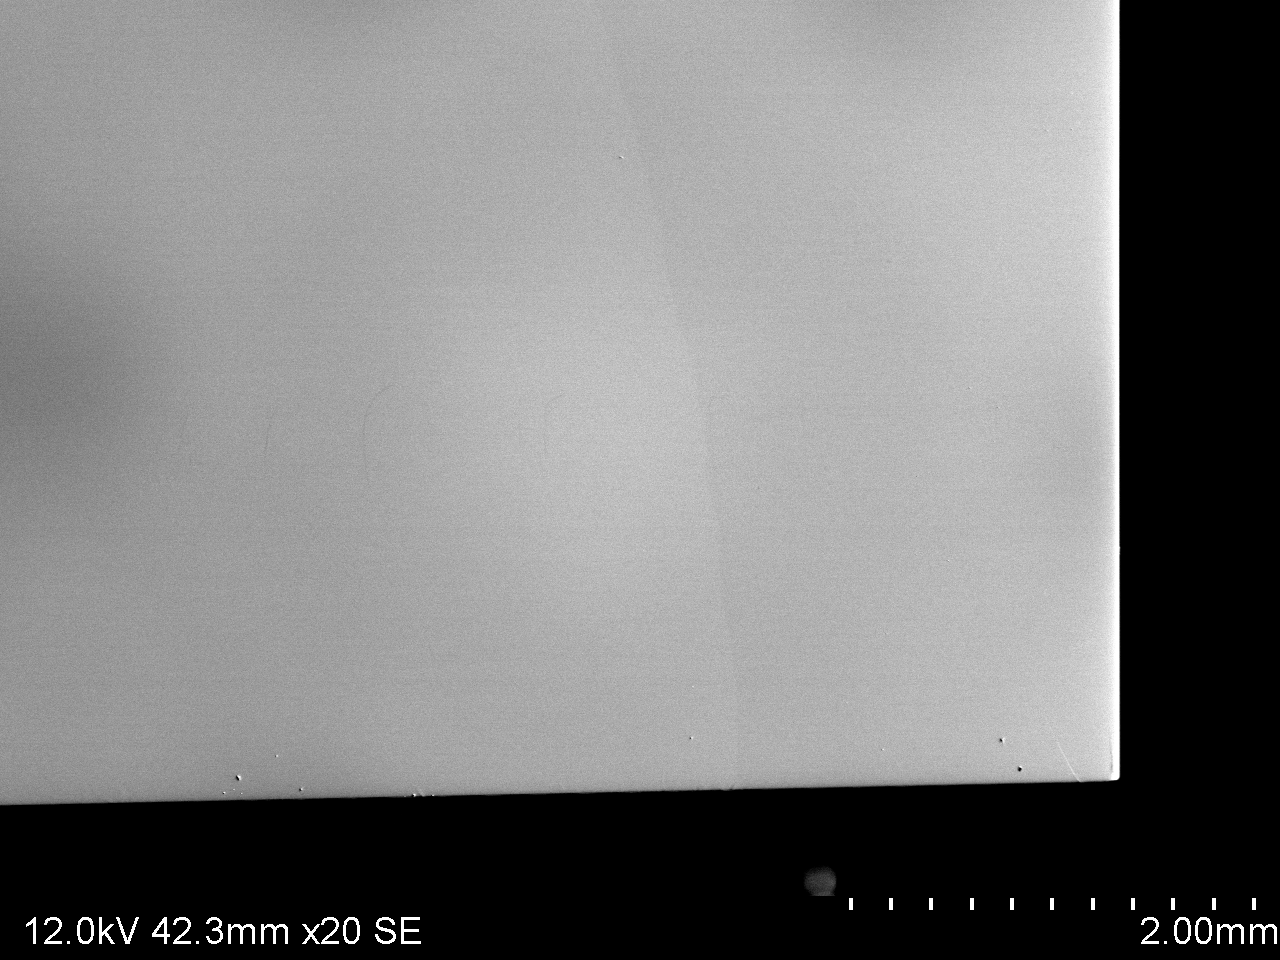
\includegraphics[width=1.0\linewidth]{subB2b_sem_05_m003.png}\caption{Right edge}
    \caption[\Ac{sem} image of the semicircle with low \ac{ir} transmission on substrate B2.]{\Ac{sem} image of the \subref{fig:subB2b_sem_low_transmission_left} left and \subref{fig:subB2b_sem_low_transmission_right} right edge of the semicircle with low \ac{ir} transmission in the lower part of substrate B2. The semicircle appears brighter than the rest of the substrate surface.}\label{fig:subB2b_sem_low_transmission}
\end{figure}

It could be different crystal orientation that caused the contrast in the \ac{sem} images in Fig.~\ref{fig:subB2b_sem_low_transmission}. \Ac{lpe} growth is particularly sensitive for the crystal orientation of the substrate (E. Selvig, personal communication, May 24, 2017). However, the films which were grown on this kind of low-transmission areas were not affected, and hence, it had likely not a different crystal orientation.

Another explanation could be that there was an absorbing layer of some sort on the surface, but as the low-transmission area was present after polishing and an etch had been performed on substrate B2, an absorbing layer was likely not the case. However, this could be investigated further by using a low \ac{eds} voltage to get higher surface sensitivity.

\citet{sealy2000mechanism} showed that p-type semiconductors in general appeared brighter and that n-type in general appeared darker than undoped material in \ac{sem}. The best contrast was achieved when using low voltage because then the number of electrons that escaped the sample had a stronger dependency on the doping in the sample. Doping contrast agreed with the expected concentration of free carriers for the sloping spectra, which was observed at the low-transmission semicircle.

Near-\ac{ir} microscopy images of the tellurium precipitate distribution in the \ac{czt} substrate can be seen in Fig.~\ref{fig:subBa_nirt}. The images are taken outside the low-transmission area. The observation of \ce{Te} precipitates contradict the analysis of \citeauthor{yujie2004infrared}. A series of 11 near-\ac{ir} microscopy images focusing through the complete depth of the substrate was acquired, each image was \SI{\sim80}{\micro\metre} deeper into the substrate. The \ce{Te} precipitate density was rather uniform throughout the bulk of the substrate with an average of 55 \ce{Te} precipitates in focus per near-\ac{ir} image. Mainly single \ce{Te} precipitates, but also some strings of \ce{Te} precipitates, were observed.

\begin{figure}[htbp]
    \centering
    \mySubfigure{0.49\linewidth}{subB2b_irt_n005b_20x_underlys_surface.png}[fig:subBa_nirt_surface]
    \hfill
    \mySubfigure{0.49\linewidth}{subB2b_irt_n005e_20x_underlys_surface-240um.png}[fig:subBa_nirt_inside]
    \caption[Near-\ac{ir} microscopy images pf \ce{Te} precipitates in substrate B.]{Near-\ac{ir} microscopy images pf \ce{Te} precipitate density and distribution near the centre of the $\SI{30}{\milli\metre}\times\SI{30}{\milli\metre}$ (111)B-oriented substrate B. Image area is $\SI{324}{\micro\metre}\times\SI{405}{\micro\metre}$. \subref{fig:subBa_nirt_surface} The (111)B surface; \subref{fig:subBa_nirt_inside} \SI{\sim240}{\micro\metre} below the (111)B surface.}\label{fig:subBa_nirt}
\end{figure}

%%========================================
